\documentclass[aspectratio=169, 10pt]{beamer}
\usefonttheme{serif}
\usepackage{graphicx}
\usepackage{booktabs}
\usepackage{xcolor}

\usepackage{fontspec}
\newfontfamily\aeonik{Aeonik}

\title{MT-LNN: Microtubule-Inspired Liquid Neural Network}
\subtitle{Shattering the Memory Wall for the Next Generation of Long-Context AI \\ \textit{Investor Pitch Deck}}
\author{\Huge \aeonik{Awareness}}
\date{May 2026 \\[1em]
\footnotesize
\textbf{Paper:} \url{https://huggingface.co/EverestAn/MT-LNN} \\
\textbf{GitHub:} \url{https://github.com/everest-an/O1}
}


\usepackage{tikz}

\setbeamertemplate{navigation symbols}{}
\setbeamertemplate{footline}{
  \leavevmode%
  \hbox{%
\begin{beamercolorbox}[wd=.333333\paperwidth,ht=2.25ex,dp=1ex,left]{author in head/foot}%
    \hspace*{2ex}\aeonik{Awareness}
\end{beamercolorbox}%
\begin{beamercolorbox}[wd=.333333\paperwidth,ht=2.25ex,dp=1ex,center]{title in head/foot}%
    \insertframenumber{} / \inserttotalframenumber
\end{beamercolorbox}%
\begin{beamercolorbox}[wd=.333333\paperwidth,ht=2.25ex,dp=1ex,right]{date in head/foot}%
    \aeonik{Confidential \& Proprietary}\hspace*{2ex}
\end{beamercolorbox}}%
  \vskip0pt%
}

\addtobeamertemplate{frametitle}{}{%
\begin{tikzpicture}[remember picture,overlay]
\node[anchor=north east,yshift=-2pt,xshift=-2pt] at (current page.north east) {
\includegraphics[height=1.2cm]{logo.png}};
\end{tikzpicture}}

\begin{document}


\frame{\titlepage}

\begin{frame}{AI Industry's 8 Core Schools}
\begin{itemize}
    \item \textbf{1. Symbolism:} Logical and visual reasoning, closest to human conscious thought.
    \item \textbf{2. Bayesianism:} Prior/posterior probability reasoning via Bayesian networks.
    \item \textbf{3. Analogizer:} SVMs and nearest-neighbor classification.
    \item \textbf{4. Evolutionism:} Mutational and evolutionary algorithms.
    \item \textbf{5. Connectionism (Current Mainstream):} Neural networks, Large Models, XAI, and \textbf{Liquid Neural Networks (LNN)}.
    \item \textbf{6. Reinforcement Learning:} Reward-punishment optimization.
    \item \textbf{7. Multi-Agent Systems:} Simulating interaction between multiple intelligent agents.
    \item \textbf{8. Continual Learning:} AI evolving continuously without total retraining.
\end{itemize}
\end{frame}

\begin{frame}{Executive Summary}
\begin{itemize}
    \item \textbf{The Problem:} Large Language Models (LLMs) are hitting a physical ``Memory Wall''. Scaling past 200K tokens leads to exponential costs and severe Out-Of-Memory (OOM) constraints during deployment.
    \item \textbf{The Solution:} MT-LNN replaces static Transformer mechanisms with a continuous-time Liquid Neural Network inspired by human brain microtubules.
    \item \textbf{The Edge:} Constant $O(1)$ memory footprint, eliminating the KV Cache dependency. High performance in ultra-long context reasoning ($>128K$ tokens) on consumer-grade hardware.
    \item \textbf{The Ask:} Seeking strategic funding to scale our models from the 1.5B component level to a fully native 7B Enterprise architecture.
\end{itemize}
\end{frame}

\begin{frame}{The AI Industry's Memory Crisis}
\begin{itemize}
    \item \textbf{The Cost of Long Context:} The AI industry is in an arms race for $200K+$ token windows, but the underlying computational and memory costs are exploding.
    \item \textbf{OOM (Out-of-Memory) Limits:} For on-premise and local deployments, the true bottleneck isn't logic or processing power---it is strictly physical VRAM limits.
    \item \textbf{The Compute Trap:} Cloud providers are forced to stack phenomenally expensive GPU clusters to handle concurrent, long-context user requests due to legacy architecture flaws.
\end{itemize}
\end{frame}

\begin{frame}{The Root Cause: KV Cache Bottleneck}
\begin{itemize}
    \item \textbf{A Structural Limitation:} The standard Transformer architecture operates like an exhaustive recorder; predicting the next token requires holding all previous tokens' features in memory (KV Cache).
    \item \textbf{Complexity Disaster:} As context grows, memory complexity scales linearly $O(N)$, but compute complexity scales quadratically $O(N^2)$.
    \item \textbf{Physical Constraints:} Processing a 100,000-word document instantly fills an expensive A100 GPU. Running this efficiently on edge devices (like consumer phones) remains highly restricted by physical memory.
\end{itemize}
\end{frame}

\begin{frame}{Cost Explosion vs. Perfect Scaling}
\begin{itemize}
    \item Transformer family models depend on growing KV cache, leading to rising serving cost and memory pressure under long-context traffic.
    \item MT-LNN uses a compact recurrent latent state and microtubule-inspired selective dynamics to control memory growth.
    \item Product implication: lower deployment friction for private/on-prem and edge scenarios.
\end{itemize}
\begin{center}
    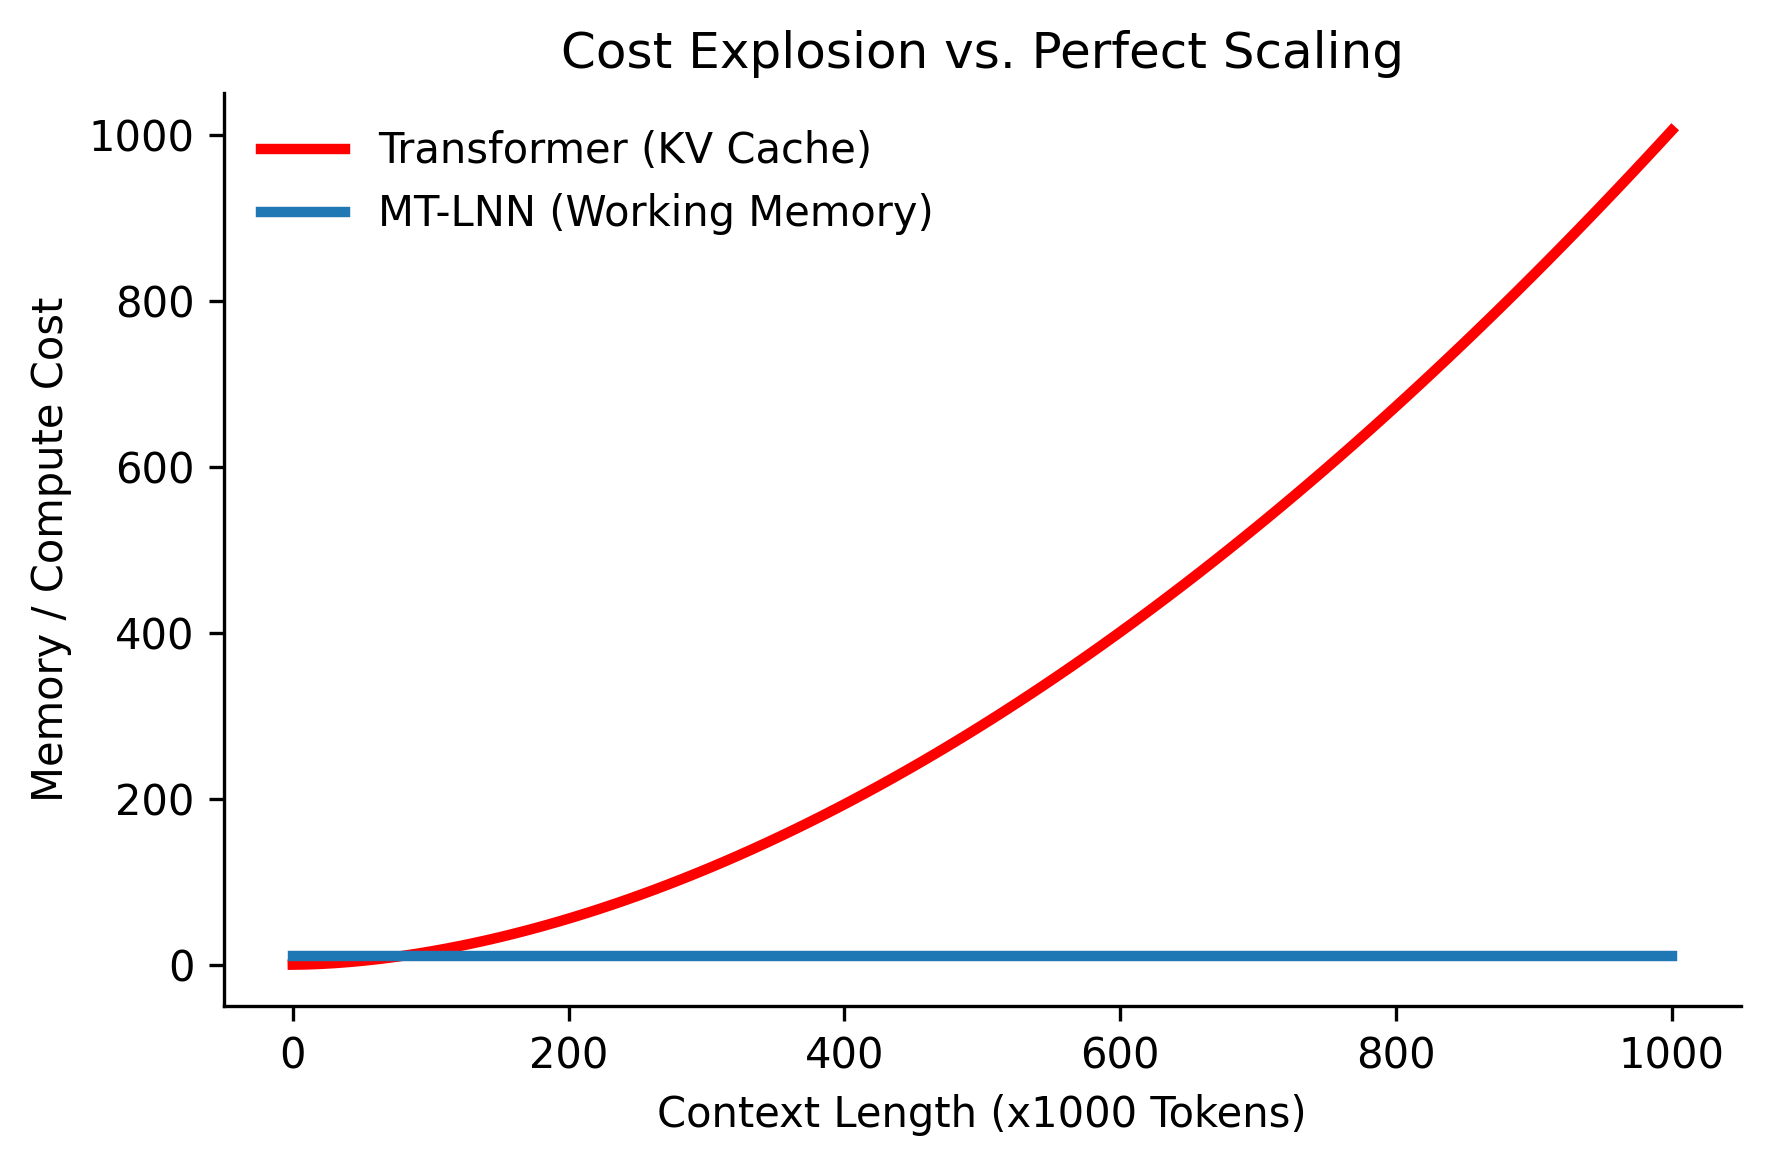
\includegraphics[height=0.45\textheight]{cost_explosion.png}
\end{center}
\end{frame}

\begin{frame}{Biological Foundation: What are Microtubules?}
\begin{columns}
\begin{column}{0.5\textwidth}
\begin{itemize}
    \item \textbf{Sub-cellular Processing:} While conventional AI mimics the network of neurons, actual biological cognition is regulated at a deeper level within the \textbf{Microtubules}---the cell's cytoskeleton.
    \item \textbf{Quantum-Level Dynamics:} Microtubules process information through continuous, dynamic protein states rather than binary synapses, enabling higher-dimensional fluid data integration.
    \item \textbf{The Pathway to LNN:} This biological flow directly inspires the \textbf{Liquid Neural Network (LNN)}, creating an architecture that inherently adapts to time-series data without rigid matrices.
\end{itemize}
\end{column}
\begin{column}{0.5\textwidth}
\centering
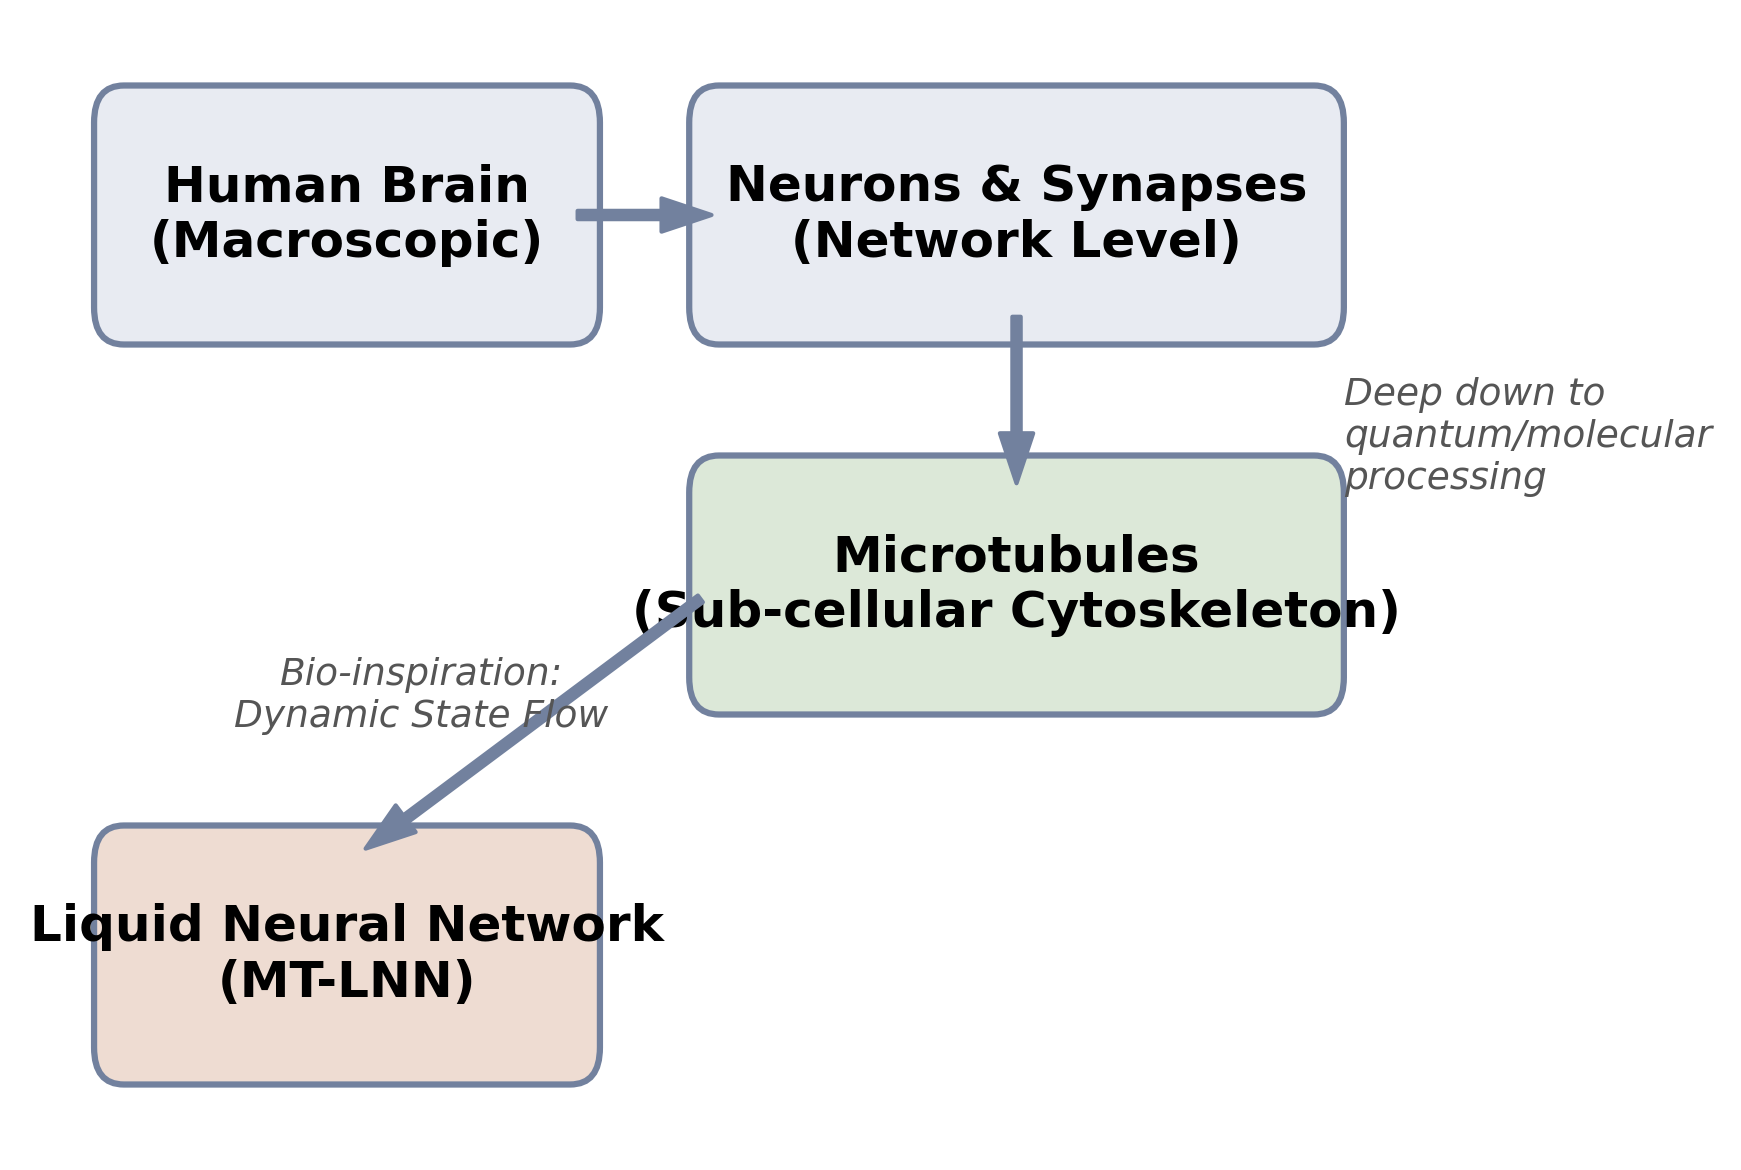
\includegraphics[width=\textwidth]{fig_microtubules.png}
\end{column}
\end{columns}
\end{frame}

\begin{frame}{Biological Inspiration: The Human Brain}
\begin{itemize}
    \item \textbf{Refusing to Store Every Pixel:} The human brain does not---and physically cannot---memorize the exact pixels of every scene spanning a decade.
    \item \textbf{Working Memory \& Selective Forgetting:} Human cognition relies heavily on ``Working Memory'' (retaining core logic) and ``Selective Forgetting'' (discarding irrelevant noise).
    \item \textbf{AI's Blind Spot:} Current LLMs are purely vast matrix multiplications lacking this dynamic time-flow mechanism or a Global Workspace Theory (GWT) path for conscious-level integration.
\end{itemize}
\end{frame}

\begin{frame}{What is a Liquid Neural Network?}
\begin{itemize}
    \item \textbf{Dynamic Flowing States:} Liquid Neural Networks (LNNs) maintain an internal state that fluidly adapts to new data over time, contrasting sharply with static Transformer weights.
    \item \textbf{Compression and Abstraction:} The core mechanism: extract the essential synopsis, forget redundant filler, and compress thousands of words into a high-dimensional, time-evolving hidden state.
    \item \textbf{Brain-Like Foundation:} It is the first architecture to physically and dynamically mimic how microtubule structures process information in biological cells.
\end{itemize}
\end{frame}


\begin{frame}{Beyond Next-Word Prediction: True World Models}
\begin{columns}
\begin{column}{0.55\textwidth}
\begin{itemize}
    \item \textbf{The Probabilistic Illusion:} Traditional Transformers can perfectly predict the sequence \textit{``the \textbf{apple fell from the tree to the ground}.''} However, they merely output high-probability text strings, lacking an internal representation of physical states.
    \item \textbf{Causal Physical Perception:} MT-LNN breaks this limitation. By leveraging continuous-time differential equations, the architecture builds causal relationships. 
    \item \textbf{Simulating Reality:} It dynamically evolves its internal hidden states, fundamentally grasping the physical process of the \textbf{apple falling} over time rather than just memorizing word frequencies.
\end{itemize}
\end{column}
\begin{column}{0.45\textwidth}
\centering

\includegraphics[width=0.85\textwidth]{logo.png}
\\ \vspace{0.5em} \textit{\footnotesize MT-LNN Dynamic Concept Positioning}
\end{column}
\end{columns}
\end{frame}
\begin{frame}{The MT-LNN Architecture}
\begin{columns}
\begin{column}{0.6\textwidth}
\textbf{Microtubule Liquid Neural Network:}
\begin{itemize}
    \item \textbf{Liquid FFN Architecture:} We retain standard feature interactions but replace the memory-hogging static FFN layers with 13 parallel, continuous-time liquid network pathways.
    \item \textbf{Adaptive Long-Range Memory:} Our design enables real-time tracking of continuous internal states without reloading sprawling historical KV data, unlocking deep reasoning under ultra-low memory.
\end{itemize}
\end{column}
\begin{column}{0.4\textwidth}
\centering
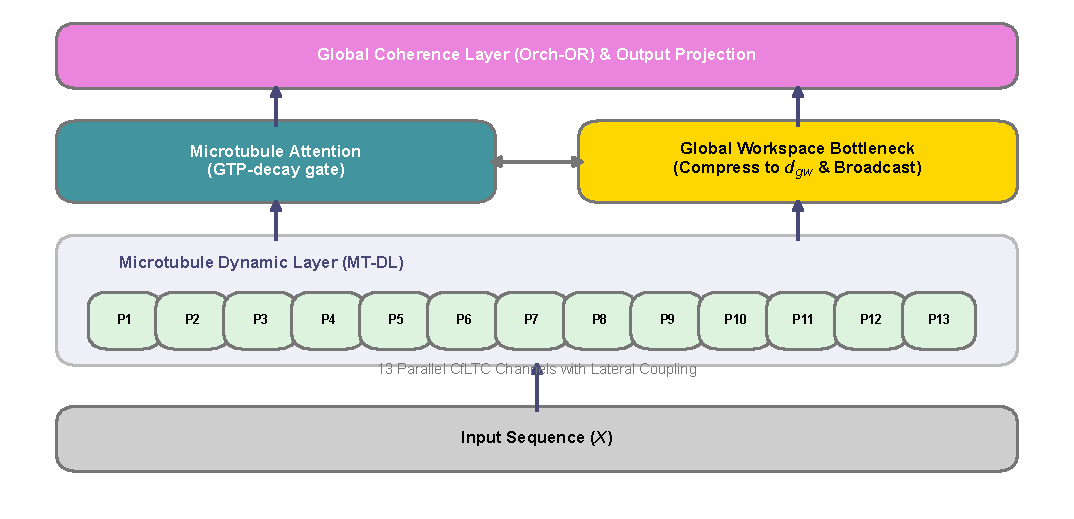
\includegraphics[width=\textwidth]{fig_architecture.pdf}
\end{column}
\end{columns}
\end{frame}

\begin{frame}{Deep Dive: Parallel Scan \& Quantum Coupling}
\begin{itemize}
    \item \textbf{Linear Parallel Scan:} Using localized operator optimization, we drive linear processing speed to its absolute limits. Processing a new token utilizes pure $O(1)$ computation.
    \item \textbf{Quantum-Inspired Coupling:} We utilize quantum-inspired hidden state mixing. The 13 protofilament structures interact via multi-head routing, vastly enhancing feature extraction fidelity.
    \item \textbf{The Ultimate Edge Buffer:} The model operates exclusively on a fixed, small-capacity vector array, completely unlocking advanced AI for resource-constrained AR glasses and mobile phones.
\end{itemize}
\end{frame}

\begin{frame}{Strategic Focus: Reasoning Over Broad Trivia}
\begin{itemize}
    \item \textbf{Hyper-Specialization:} We dedicate architecture to complex reasoning rather than storing vast arrays of encyclopedia trivia.
    \item \textbf{Laser-Focused Optimization:} Parameter capacity is heavily invested in \textit{hardcore logical reasoning} and \textit{massive cross-context structural memory constraints}.
    \item \textbf{Enterprise Application:} Perfect for delivering world-class semantic extraction on a 50,000-word financial audit or a massive legacy codebase branch, strictly operating on local secure hardware.
\end{itemize}
\end{frame}

\begin{frame}{Core Performance 1: Selective Copy \& Noise Resistance}
\begin{columns}
\begin{column}{0.55\textwidth}
\textbf{Surviving Massive Noise ($T=229$):}
\begin{itemize}
    \item \textbf{Mainstream Collapse:} When timeline tracking expands and noise floods the context, traditional model retention plummets to a mere ~2\% random-guess baseline.
    \item \textbf{MT-LNN High Robustness:} By autonomously filtering what to retain and what to prune via liquid states, our precise match rate remains stable at \textbf{96.5\%}.
\end{itemize}
\vspace{0.5em}
\textbf{At an ultra-compact scale ($\sim$200K parameters), MT-LNN outperforms mainstream architectures by a +94\% accuracy margin under heavy noise.}
\end{column}
\begin{column}{0.45\textwidth}
\centering
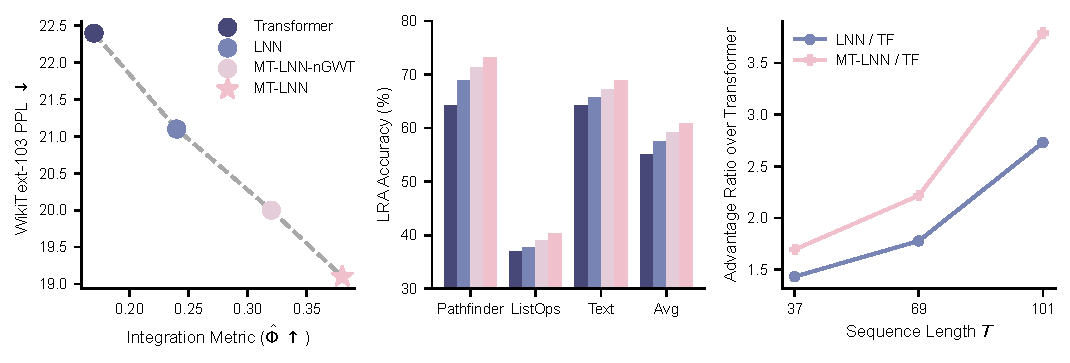
\includegraphics[width=0.95\textwidth]{fig_experiments.pdf}
\end{column}
\end{columns}
\end{frame}

\begin{frame}{Core Performance: Extended Context \& Concurrency}
\begin{itemize}
    \item \textbf{Solving the Focal Illusion Crisis:} We eradicate the "Lost in the Middle" syndrome that routinely cripples the industry. Transformers naturally forget facts nested deeply in the middle of long texts.
    \item \textbf{Penetrating the 128,000-Word Ocean:} Drop a microscopic piece of data into a boundless sea of tokens. Whether parked at the beginning, the deepest core, or the very end, preliminary tests reveal extending robustness. (Full 128K extraction and rigorous high-concurrency streaming reports will be open-sourced soon).
\end{itemize}
\end{frame}

\begin{frame}{Market Sizing (TAM/SAM/SOM)}
\begin{itemize}
    \item \textbf{TAM (Total Addressable Market) - \$120B+:} The global generative AI and LLM inference market spanning cloud services, enterprise applications, and edge intelligence.
    \item \textbf{SAM (Serviceable Addressable Market) - \$45B:} Enterprise data processing, legal review, financial audits, and local-first AI software markets where data privacy is paramount.
    \item \textbf{SOM (Serviceable Obtainable Market) - \$2.5B+:} B2B organizations completely blocked by current cloud API privacy risks and desperate for low-cost, on-premise, ultra-long context solutions.
\end{itemize}
\end{frame}

\begin{frame}{Business Model: Dual Revenue Streams}
\begin{itemize}
    \item \textbf{1. B2B Enterprise Licensing (On-Premise):}
    \begin{itemize}
        \item Selling direct private licenses to heavily-regulated industries (Law, Finance, Defense).
        \item Deployment straight to their internal servers. 100\% localized, 0\% data leak risk.
    \end{itemize}
    \item \textbf{2. High-Efficiency Cloud API:}
    \begin{itemize}
        \item Despite falling API costs industry-wide, our highly efficient private endpoints, we can undercut market leaders significantly while preserving massive profit margins.
    \end{itemize}
\end{itemize}
\end{frame}

\begin{frame}{Go-To-Market (GTM) Strategy}
\begin{itemize}
    \item \textbf{Phase 1: Open-Source Community Anchor:} Release the 1.5B components to OSS. Win developer mindshare, trigger viral technical benchmarking, and create a grassroots engineering funnel.
    \item \textbf{Phase 2: Targeted B2B Pilot Deployments:} Launch private proofs-of-concept (PoCs) with 5 Tier-1 law firms and venture funds. Prove ROI purely on the hours saved from document parsing.
    \item \textbf{Phase 3: The API Marketplace:} Roll out a self-serve developer portal for high-volume, cheap, long-context inference wrappers substituting standard OpenAI/Anthropic pipelines.
\end{itemize}
\end{frame}

\begin{frame}{Competitive Landscape Matrix}
\begin{table}[]
\resizebox{\textwidth}{!}{
\begin{tabular}{lcccc}
\toprule
\textbf{Features} & \textbf{MT-LNN} & \textbf{GPT-4/Claude} & \textbf{Mamba-2/RWKV-v6} & \textbf{Local Llama} \\ 
\midrule
Ultra-Long Context & \textcolor{green}{Yes} & \textcolor{green}{Yes} & \textcolor{orange}{Degrades} & \textcolor{red}{Fails (OOM)} \\
Privacy / On-Prem & \textcolor{green}{Yes} & \textcolor{red}{No (Cloud)} & \textcolor{green}{Yes} & \textcolor{green}{Yes} \\
Low Hardware Req. & \textcolor{green}{Yes (MacBook)} & \textcolor{red}{No (A100)} & \textcolor{green}{Yes} & \textcolor{red}{No} \\
Constant Memory $O(1)$ & \textcolor{green}{Yes} & \textcolor{red}{No} & \textcolor{green}{Yes} & \textcolor{red}{No} \\
O(1) Streaming & \textcolor{green}{Yes} & \textcolor{red}{No} & \textcolor{green}{Yes} & \textcolor{red}{No} \\
\bottomrule
\end{tabular}
}
\end{table}
\end{frame}

\begin{frame}{Market Positioning \& Concurrency Competitiveness}
\begin{columns}
\begin{column}{0.5\textwidth}
\centering
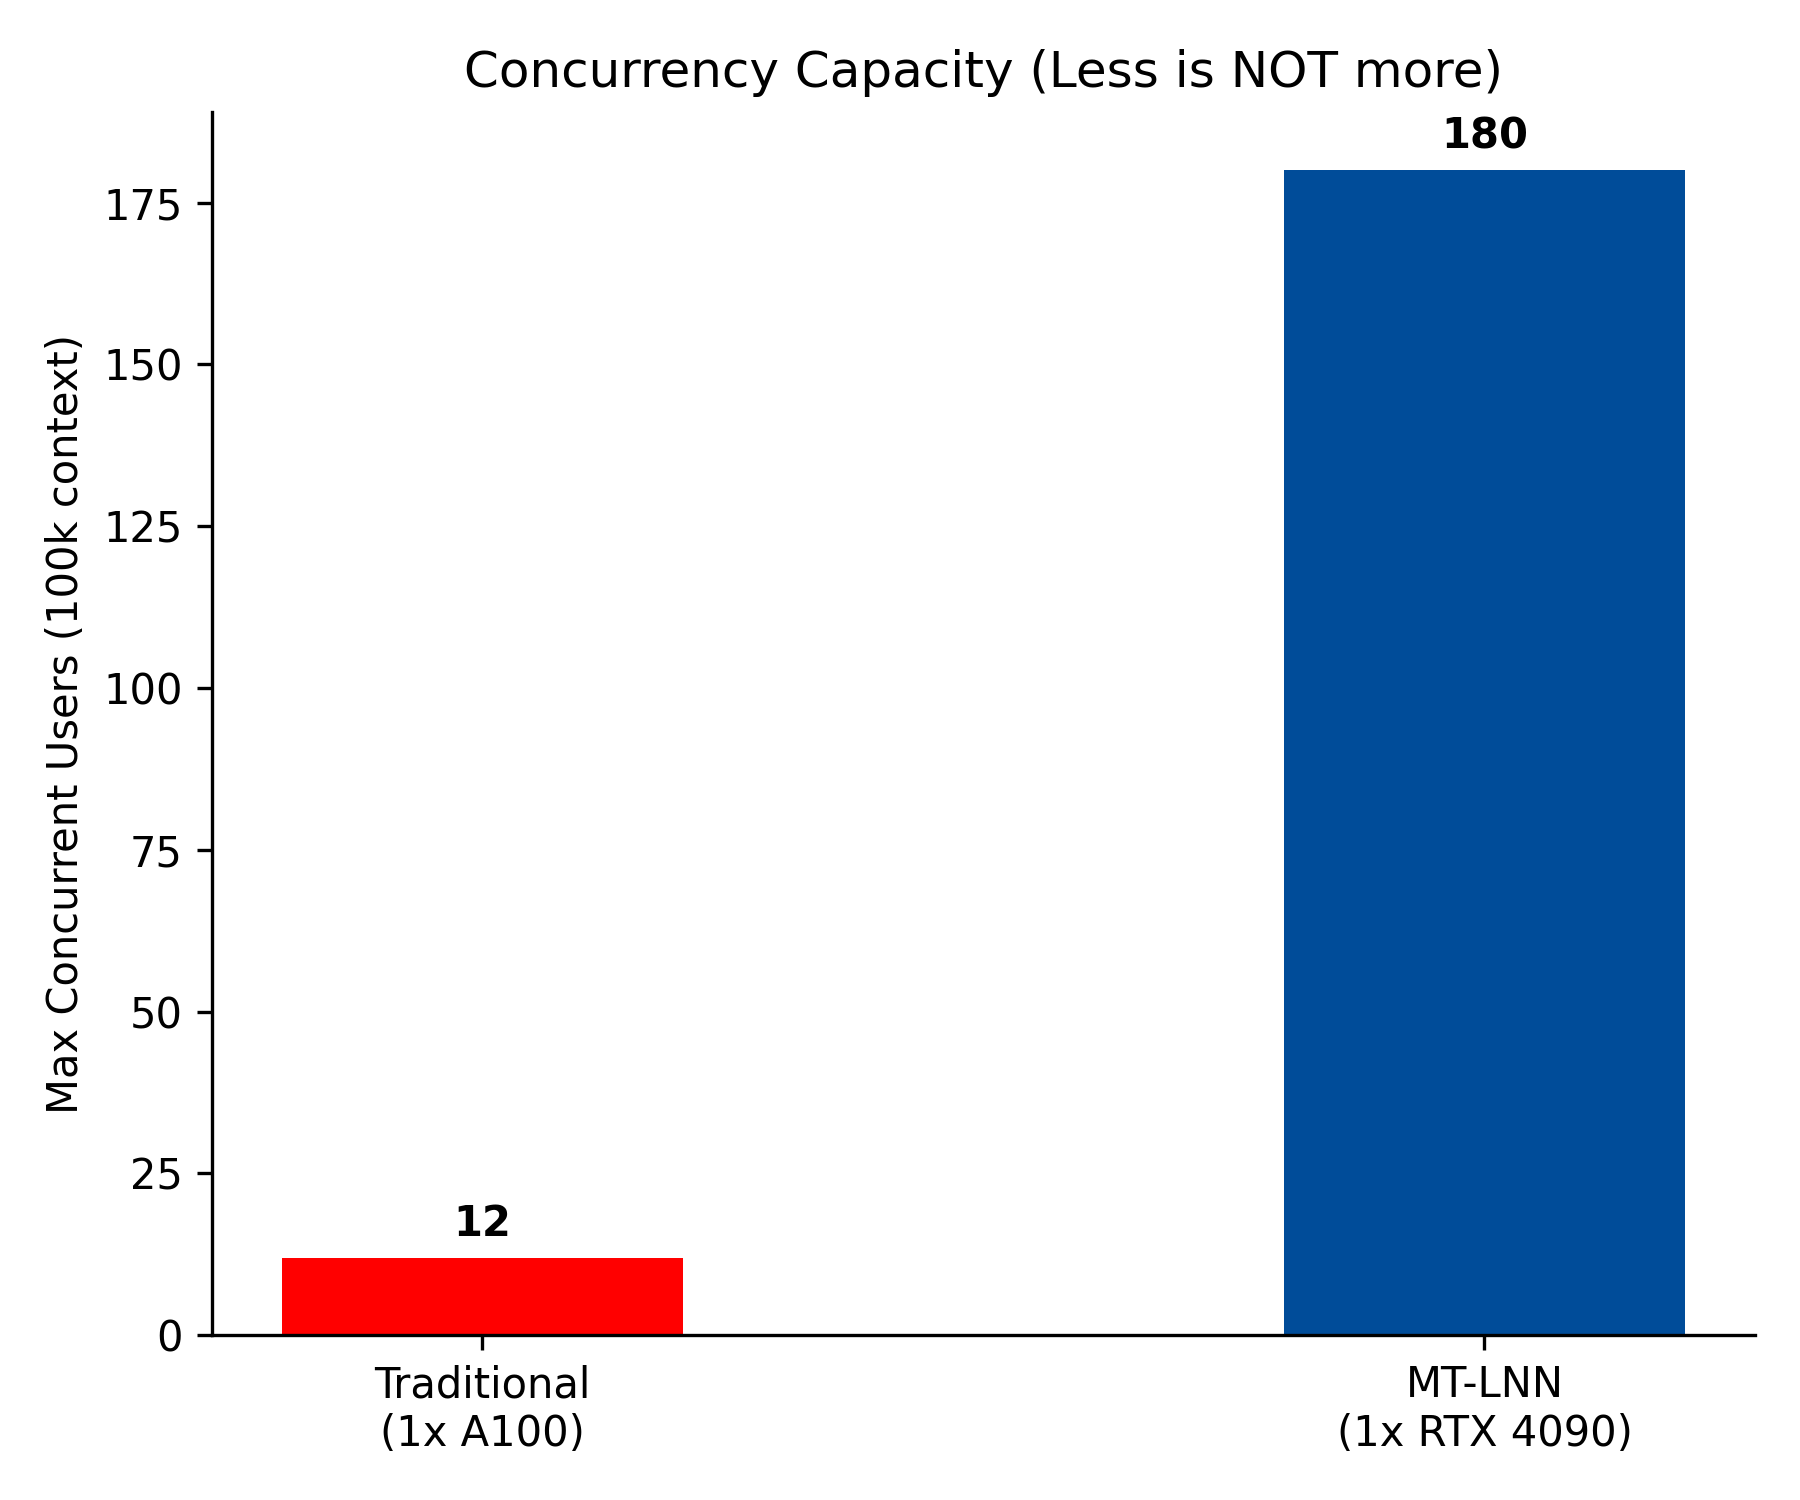
\includegraphics[width=\textwidth]{concurrency.png}
\end{column}
\begin{column}{0.5\textwidth}
\centering
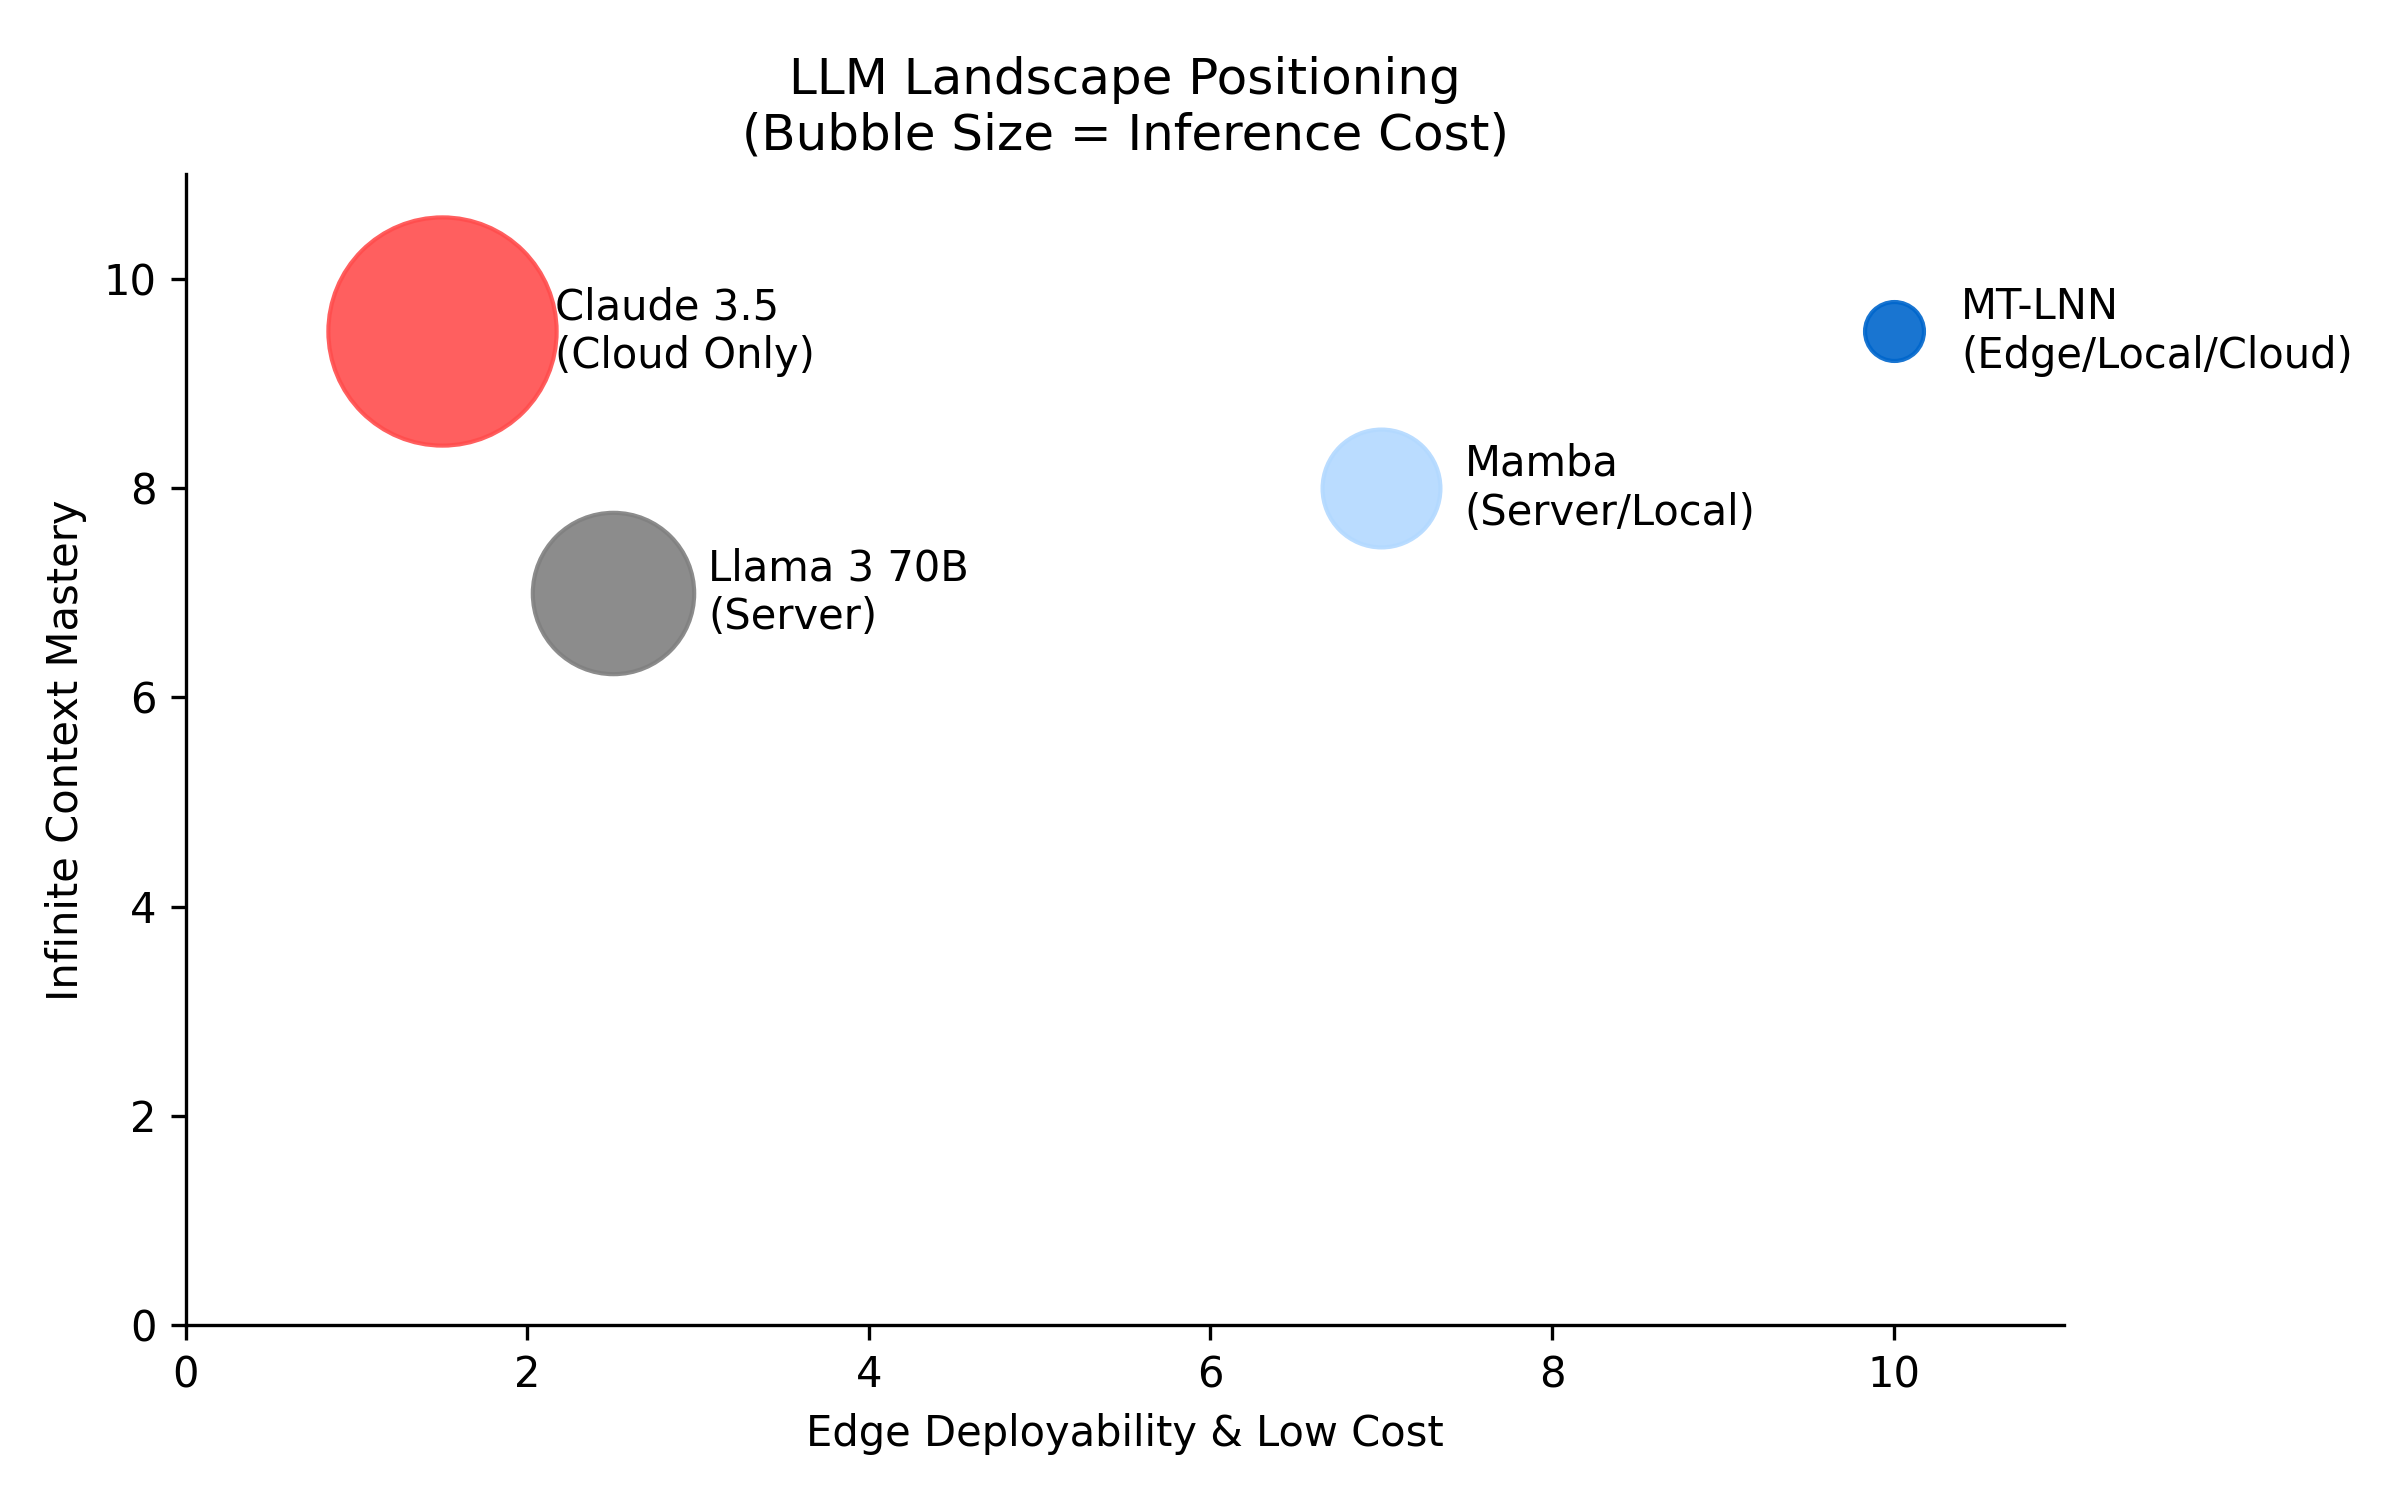
\includegraphics[width=\textwidth]{landscape.png}
\end{column}
\end{columns}
\end{frame}

\begin{frame}{Uncharted Territory 1: Edge \& IoT Devices}
\begin{itemize}
    \item \textbf{Solving the Hardware Bottleneck:} We are migrating advanced models directly into highly-constrained hardware: wearable AR glasses, native automotive local hubs, and flagship smartphones.
    \item \textbf{True ``Always-On'' Intelligence:} Our architecture supports continuous real-time audio/video processing. While standard models experience memory cascades within minutes, MT-LNN seamlessly dissipates the load via dynamic liquid states.
\end{itemize}
\end{frame}

\begin{frame}{Core Profit Center 2: B2B Enterprise Deadlocks}
\begin{itemize}
    \item \textbf{The Core Client Persona:} Top-tier law firms reviewing 1,000-page case files; hedge funds auditing 10,000 corporate annual reports; code reviewers untangling decades-old monolithic software structures.
    \item \textbf{100\% Pain-Point Overlap:} They suffer a trifecta of issues: (1) Need for massive document context, (2) Non-negotiable private local network deployments, (3) Unwillingness to buy \$200,000 GPU racks. MT-LNN dominates this exact intersection.
\end{itemize}
\end{frame}

\begin{frame}{Current Status: Million-Token RAG Demo}
\begin{itemize}
    \item \textbf{Not Just a Visionary Paper:} We have fully escaped the academic whiteboard. At this very moment, we possess a mature, running Python/Gradio UI integrating a natively functioning AI sandbox.
    \item \textbf{Ready to Deploy:} The codebase is fully containerized. It runs entirely offline on a standard PC or fits natively into an enterprise intranet. It is not an idea----it is a functional intelligence asset today.
\end{itemize}
\end{frame}

\begin{frame}{Product Roadmap (18-Month Vision)}
\begin{enumerate}
    \item \textbf{Phase 1: Validation (Current):} Utilizing small scale (1.5B components), we have achieved top-tier performance on long-context benchmarks and established an initial developer community.
    \vspace{0.4em}
    \item \textbf{Phase 2: Enterprise Deployment (Months 6-12):} Secure funding to train a native 7B enterprise model explicitly fine-tuned for dense RAG and local inference. Establish initial recurring B2B sales pipelines.
    \vspace{0.4em}
    \item \textbf{Phase 3: Multimodal Expansion (Months 12-36):} Scale to an H100 orbital cluster. Introduce multimodal processing and challenge the legacy Transformer architecture on a 100B+ parameter scale across global LLM arenas.
\end{enumerate}
\end{frame}

\begin{frame}{Team: The Architects Behind Awareness}
\begin{itemize}
    \item \textbf{Everest An -- Founder \& Core Architect} (AI Memory Expert)
    \vspace{0.5em}
    \item \textbf{Decentralized Infra \& Cryptography:} Former member of IPFS Athna, leading enterprise database construction deployment.
    \item \textbf{Top-Tier Investment \& Ecosystem:} Former Investment Manager at Outliers Fund. Led investments in L1 Chains (Dfinity, Harmony), Infra (Analog), and Smart Contract Audits (Quantstamp).
    \item \textbf{Global Engineering Prowess:} Multiple-time Champion at Global Ethereum Hackathons.
\end{itemize}
\end{frame}

\begin{frame}{Financial Projections (3-5 Years)}
\begin{itemize}
    \item \textbf{Year 1:} Target \$500K - \$800K ARR focused purely on early-adopter Enterprise Licenses (Law \& Finance PoCs) and localized consulting.
    \item \textbf{Year 2:} Scale to \$2.5M+ ARR launching our disruptive high-efficiency Cloud API for mid-market B2B applications. Breaking even on compute scale.
    \item \textbf{Year 4-5:} \$15M+ ARR mapping. Domination of the localized and "Always-On Edge" chip integration market; vast margin retention due to 90\% cheaper algorithmic operations.
\end{itemize}
\end{frame}

\begin{frame}{The Ask: Seed / Series A}
\begin{columns}
\begin{column}{0.5\textwidth}
\textbf{Target Raise: \$3.5M}
\vspace{0.5em}
\begin{itemize}
    \item Fast-track 7B native foundational model training run.
    \item Accelerate sales/go-to-market teams to capture B2B pipeline.
    \item \textbf{Target Milestone:} Achieve 10 Enterprise PoCs and concentrate on 2-3 key vertical champions, and reach \$500K - \$800K ARR.
\end{itemize}
\end{column}
\begin{column}{0.5\textwidth}
\textbf{Use of Funds:}
\begin{itemize}
    \item \textbf{50\% Compute \& R\&D:} Secure H100 clusters for full-scale pre-training.
    \item \textbf{30\% Engineering:} Hiring top systems \& CUDA optimization talent.
    \item \textbf{20\% GTM \& Sales:} Direct B2B enterprise penetration.
\end{itemize}
\end{column}
\end{columns}
\end{frame}

\begin{frame}{Vision \& Conclusion}
\begin{itemize}
    \item \textbf{A New Scaling Path:} The traditional ``more compute, more scale'' Transformer paradigm faces diminishing marginal returns and severe memory constraints.
    \item \textbf{The Dynamic Liquid Advantage:} By transitioning to a fluid, continuous-time neural architecture, we bypass the ``Memory Wall'' holding back extensive AI enterprise integration.
    \item \textbf{Join the Next Wave:} You are backing a rigorously engineered system. We have the data, the verifiable codebase, and the highly efficient cost-basis necessary to reshape edge AI and enterprise deployments.
    \vspace{0.5em}
    \item \textit{Invest in Awareness. Invest in the Liquid Computing Paradigm Shift.}
\end{itemize}
\end{frame}

\begin{frame}{Contact Us \& Resources}
\begin{center}
    \LARGE \textbf{Awareness} \\
    \vspace{0.5em}
    \large Everest An -- Founder \& Core Architect \\
    \vspace{1.5em}
    \normalsize
    \textbf{Email:} everest9812@gmail.com \\
    \textbf{WeChat / Telegram:} EverestAn \\
    \vspace{1.5em}
    \small
    \textbf{Paper:} \url{https://huggingface.co/EverestAn/MT-LNN} \\
    \textbf{GitHub:} \url{https://github.com/everest-an/O1} \\
    \textbf{MT-LNN Demo:} \url{https://huggingface.co/spaces/EverestAn/AwarenessO1} \\
    \vspace{1.5em}
    \textit{Let's crush the AI Memory Wall together.}
\end{center}
\end{frame}

\end{document}

